\documentclass[aspectratio=1610]{beamer}
\setbeamersize{text margin left=7mm,text margin right=5mm}
\usefonttheme[onlymath]{serif}
\usetheme{default}
\usefonttheme{professionalfonts}
%\setbeamertemplate{navigation symbols}{} 
\beamertemplatenavigationsymbolsempty
\addtobeamertemplate{navigation symbols}{}{
    \usebeamerfont{footline}
    \usebeamercolor[fg]{footline}
    %\hspace{1em}
    \footnotesize\insertframenumber\,%/\inserttotalframenumber
}

\usepackage[round]{natbib}
%\bibliographystyle{plainnatnourl} 

% cSpell:disable
\definecolor{rcomment}{rgb}{0.3, 0.3, 0.3}  % darkgrey
\definecolor{rred}{rgb}{0.7,0.2,0.2}        % red
\definecolor{rblue}{rgb}{0.2,0.2,0.7}       % blue (blended blue of beamer)
\definecolor{rpurple}{rgb}{0.45, 0.0, 0.9}  % violett
\definecolor{rpink}{rgb}{0.8, 0.0, 0.4}     % pink
\definecolor{rgreen}{rgb}{0.1, 0.5, 0.1}    % darkgreen
\definecolor{rorange}{rgb}{0.8, 0.4,0}      % orange
\definecolor{rblack}{rgb}{0, 0, 0}          % black
\definecolor{deeptuerkis}{rgb}{0, 0.5, 0.5} % Türkis
\definecolor{darkgreen}{rgb}{0,0.5,0}
\definecolor{blendedblue}{rgb}{0.2,0.2,0.7}
\newcommand{\important}[1]{{\color{green!60!black}#1}}


% \documentclass{beamer}
% \mode<presentation> {
%   \usetheme{Singapore}
%   \setbeamertemplate{navigation symbols}{}
%   \setbeamertemplate{footline}[frame number]
% }

\usepackage[utf8]{inputenc}
\usepackage{caption}
\usepackage{nicefrac}
\usepackage{varwidth}
\usepackage{amsmath}
\usepackage{hyperref}
\usepackage{color}
\usepackage{xcolor}
\usepackage[linesnumbered, ruled, noend]{algorithm2e}
\usepackage{appendixnumberbeamer}
\usepackage{booktabs}
\usepackage{multirow}


\usepackage{natbib}
% \usepackage[backend=bibtex,style=authoryear-comp]{biblatex}
% \bibliography{bibliography}

\usepackage[draft,nomargin,inline]{fixme}  % add final for disabling remarks
\fxsetface{inline}{\itshape}
\fxsetface{env}{\itshape}
%\fxuselayouts{margin}
%\fxuselayouts{inline}
\fxusetheme{color}

\usepackage{tikz}
\usepackage{pgfplots}
\usetikzlibrary{calc, decorations.markings}
\tikzset{vertex/.style={circle, draw=black}}
\tikzset{tr/.style={draw=white, fill=white, sloped}}
\tikzset{del/.style={draw=red, text=red}}
\tikzset{layer/.style={rectangle, draw=black, minimum width=1.5cm, minimum height=0.75cm}}
\tikzset{plus/.style={
  circle, draw=black, minimum width=0.3cm, inner sep=0cm, outer sep=0cm,
  path picture={
    \draw[black] (path picture bounding box.south) -- (path picture bounding box.north)
                 (path picture bounding box.west) -- (path picture bounding box.east);
  }
}}
\tikzset{buswidth/.style={decoration={
  markings,
  mark=at position 0.5 with {\node[font=\footnotesize] {/};\node[below=3pt] {\tiny #1};}
}, postaction={decorate}}}

\pgfplotsset{compat=1.18}


\newcommand{\tmax}{\ensuremath{t^\mathrm{max}}}
\newcommand{\plim}{\ensuremath{p^\mathrm{lim}}}
\newcommand{\ILP}{\ensuremath{\mathrm{ILP}}}
\newcommand{\ppath}{\ensuremath{p^\mathrm{path}}}
\newcommand{\Tavail}{T^\mathrm{avail}}
\newcommand{\Irej}{I^\mathrm{rej}}
\newcommand{\Greedy}{\textsc{Greedy}}
\newcommand{\Markov}{\textsc{Markov}}

\pgfplotsset{compat=newest}
\usepgfplotslibrary{statistics}

\usepackage{tikz}
\usetikzlibrary{arrows,automata}
\usetikzlibrary{datavisualization}
\usetikzlibrary{positioning}
\usetikzlibrary{calc}
\usetikzlibrary{patterns}
\usetikzlibrary{matrix}
\usetikzlibrary{decorations.pathreplacing}
\usetikzlibrary{shapes.geometric, arrows, arrows.meta}

\tikzstyle{vertex} = [circle, draw=black, fill=black, minimum width=0.15cm, inner sep=0cm, text centered]
\tikzstyle{arc} = [thick,->,>=stealth]
\tikzstyle{emphvertex} = [circle, draw=red, fill=red, minimum width=0.15cm, inner sep=0cm, text centered]
\tikzstyle{empharc} = [thick,->,>=stealth, draw=red]
\tikzstyle{vertex-green} = [circle, draw=ForestGreen, fill=ForestGreen, minimum width=0.15cm, inner sep=0cm, text centered]
\tikzstyle{arc-green} = [very thick,->,>=stealth, draw=ForestGreen] %thick, very thick, ultra thick
\tikzstyle{bgvertex} = [circle, draw=black!40, fill=black!40, minimum width=0.15cm, inner sep=0cm, text centered]
\tikzstyle{bgarc} = [draw=black!40,thick,->,>=stealth]
\tikzstyle{move} = [thick, ->, -Implies, double,double distance=0.7mm]
\tikzstyle{cyclearc} = [thick,->,>=stealth,draw=red]
\tikzstyle{gets} = [thick, ->, -{Implies[length=5mm, width=3mm]}, double, double distance=1mm]

\usepackage{rotating}
\usepackage{subcaption}
\usepackage{cancel}

\newcommand\hcancel[2][black]{\setbox0=\hbox{$#2$}%
\rlap{\raisebox{.45\ht0}{\textcolor{#1}{\rule{\wd0}{1pt}}}}#2} 


% CHEATING DASH FROM https://tex.stackexchange.com/a/133357/128068
\tikzset{
	cheating dash/.code args={on #1 off #2}{
		% Use csname so catcode of @ doesn't have do be changed.
		\csname tikz@addoption\endcsname{%
			\pgfgetpath\currentpath%
			\pgfprocessround{\currentpath}{\currentpath}%
			\csname pgf@decorate@parsesoftpath\endcsname{\currentpath}{\currentpath}%
			\pgfmathparse{\csname pgf@decorate@totalpathlength\endcsname-#1}\let\rest=\pgfmathresult%
			\pgfmathparse{#1+#2}\let\onoff=\pgfmathresult%
			\pgfmathparse{max(floor(\rest/\onoff), 1)}\let\nfullonoff=\pgfmathresult%
			\pgfmathparse{max((\rest-\onoff*\nfullonoff)/\nfullonoff+#2, #2)}\let\offexpand=\pgfmathresult%
			\pgfsetdash{{#1}{\offexpand}}{0pt}}%
	}
}


\usepackage[normalem]{ulem} % for strikethrough text
\newcommand\soutred{\bgroup\markoverwith{\textcolor{red}{\rule[0.5ex]{2pt}{0.4pt}}}\ULon} % for crossing out text in red


%******************************
%rest of frame
\usepackage{zref-savepos}

\newcounter{restofframe}
\newsavebox{\restofframebox}
\newlength{\mylowermargin}
\setlength{\mylowermargin}{2pt}

\newenvironment{restofframe}{%
	\par\centering
	\stepcounter{restofframe}%
	\zsavepos{restofframe-\arabic{restofframe}-begin}%
	\begin{lrbox}{\restofframebox}%
	}{%
\end{lrbox}%
\setkeys{Gin}{keepaspectratio}%
\raisebox{\dimexpr-\height+\ht\strutbox\relax}[0pt][0pt]{%
	\resizebox*{!}{\dimexpr\zposy{restofframe-\arabic{restofframe}-begin}sp-\zposy{restofframe-\arabic{restofframe}-end}sp-\mylowermargin\relax}%
	{\usebox{\restofframebox}}%
}%
\vskip0pt plus 1filll\relax
\mbox{\zsavepos{restofframe-\arabic{restofframe}-end}}%
\par 
}

\let\oldfootnotesize\footnotesize
\renewcommand*{\footnotesize}{\oldfootnotesize\fontsize{6}{4}\selectfont}

% reset footnote counter for each frame
\AtBeginEnvironment{frame}{\setcounter{footnote}{0}}

% command for bold blue text
%\DeclareTextFontCommand{\structure}{\color{TuWienBlue}\bfseries}



% \renewcommand{\thefootnote}{\fnsymbol{footnote}}
% cSpell:enable

\title{Advances in Large Neighborhood Search \\for Electric Dial-A-Ride Problems and in\\ Logic-Based Benders Decomposition for Scheduling Problems
}

\author{Günther R.\ Raidl}
\date{University of Auckland, NZ\\March 9, 2025}
\titlegraphic{\includegraphics[height=7mm]{graphics/logo-tuwien-informatics.png}\quad
	\includegraphics[height=7mm]{graphics/AClongColor.pdf}}

\institute[]{\normalsize Algorithms and Complexity Group, TU Wien, Austria,\\
    \texttt{raidl@ac.tuwien.ac.at}\\[1ex]
}

\logo{\includegraphics[height=15pt]{graphics/logo.pdf}\vspace{245pt}} % Logo on top right

% cSpell:disable
\definecolor{rred}{rgb}{0.7,0.2,0.2}         % red
\newcommand{\hl}[1]{\textcolor{rred}{#1}}    % highlight

\definecolor{rgreen}{rgb}{0.216,0.784,0.216} % green
\definecolor{rblue}{rgb}{0.216,0.443,0.784}  % blue
\definecolor{rorange}{rgb}{1.0,0.4,0.0}      % orange

\definecolor{orange}{RGB}{255,100,66}
\definecolor{seaborn0}{HTML}{1f77b4}
\definecolor{seaborn1}{HTML}{ff7f0e}
\definecolor{seaborn2}{HTML}{2ca02c}
\definecolor{seaborn3}{HTML}{d62728}
\definecolor{seaborn4}{HTML}{9467bd}
\definecolor{seaborn5}{HTML}{8c564b}
\definecolor{seaborn6}{HTML}{e377c2}
\definecolor{seaborn7}{HTML}{7f7f7f}
\definecolor{seaborn8}{HTML}{bcbd22}
\definecolor{seaborn9}{HTML}{17becf}

\newbool{printlegend}

\newcommand{\cumuldistr}[7]{ % Arguments: source directory, data series, width, height, x label, y label, title
  \begin{tikzpicture}
    \begin{semilogxaxis}[%
          width={#3},
          height={#4},
          title style={align=center},
          title={\large #7},
          xlabel style={at={(axis description cs:0.5,0.05)},anchor=north},
          xlabel=#5,
          ylabel style={align=center},
          ylabel=#6,
          every axis plot post/.append style={mark=none},
          every axis plot/.append style={thick},
          legend entries={GNN,Random,Sorted,Hooker},
          \ifbool{printlegend}{
            legend columns=1,
            legend pos=south east,
          }{
            legend to name=legend:cumuldistr-#1-#2,
            legend columns=-1,
          }
          ]
      \addplot+[seaborn0, solid]  table [x=#2, y=no_instances, col sep=comma, mark=none] {#1/pgdeletion_#2.csv};
      \addplot+[seaborn1, dashed] table [x=#2, y=no_instances, col sep=comma, mark=none] {#1/deletion_#2.csv};
      \addplot+[seaborn2, dashed] table [x=#2, y=no_instances, col sep=comma, mark=none] {#1/sdeletion_#2.csv};
      \addplot+[seaborn3, dashed] table [x=#2, y=no_instances, col sep=comma, mark=none] {#1/hdeletion_#2.csv};
    \end{semilogxaxis}
  \end{tikzpicture}
}
% cSpell:enable
\renewcommand{\footnotesize}{\scriptsize}

\begin{document}{}


\part{Main}

\begin{frame}
  \titlepage
\end{frame} 


\begin{frame}{Main Research Interests of G.R.}


\medskip 
\begin{minipage}{0.45\textwidth}
  \begin{itemize}
      \item Combinatorial optimization (COP)
      \item Metaheuristics
      \item Mathematical programming
      \item Constraint programming
      \item Machine learning
      \item \important{\bf Hybrid approaches} incl.\ matheuristics, learning + classical algorithms for COP
  \end{itemize}
\end{minipage}\qquad
\begin{minipage}{0.4\textwidth}
    \structure{Application areas}
    \begin{itemize}
      \item Transport optimization
      \item Scheduling
      \item Network design
      \item Problems in bioinformatics
      \item Cutting and packing
    \end{itemize}
  \end{minipage}

  \bigskip
  \includegraphics[width=\textwidth]{graphics/AC-TU-Wien.jpg}
\end{frame}


\begin{frame}{Selected Ongoing Projects}
\begin{itemize}
  \itemsep3.5ex
  \item \structure{Dynamic Vehicle Routing Problems with Focus on E-mobility \& Learning}
  \begin{itemize}
    \item with T.~Rodemann et al., Honda Research Institute Europe
    \item with Y. Mei, Victoria University of Wellington, NZ
  \end{itemize}

  \includegraphics[width=0.8\textwidth]{graphics/darp-bss-example.jpg}
\end{itemize}
\end{frame}


\begin{frame}{Selected Ongoing Projects (contd.)}
\begin{itemize}
	\itemsep3.5ex
	\item \structure{Cooperative Personnel Scheduling}
	\begin{itemize}
	\item with S.~Limmer et al., Honda Research Institute Europe
	\end{itemize}

	\includegraphics[width=0.6\textwidth]{graphics/coopsched.png}
\end{itemize}
\end{frame}
	
\begin{frame}{Selected Ongoing Projects (contd.)}
	\begin{itemize}
	  \itemsep3.5ex
	  \item \structure{Roman Domination Problems, Influence Maximization Problems, and Variants}
	  \begin{itemize}
		\item with M. Djukanovic et al., Univ.\ of Banja Luka, Bosnia and Herzegovina
	  \end{itemize}

	  \bigskip
	  \includegraphics[width=0.7\textwidth]{graphics/influence_maximization.png}
	\end{itemize}
\end{frame}
	
\begin{frame}{Selected Ongoing Projects (contd.)}
	\begin{itemize}
	  \itemsep3.5ex
	  \item Doctoral College Vienna Graduate School on Computational Optimization
	  \begin{itemize}
		\item with University of Vienna, IST Austria, Vienna University of Economics and Business
	  \end{itemize}

	  \includegraphics[width=0.5\textwidth]{graphics/vgsco.png}
	\end{itemize}
\end{frame}
	

\begin{frame}{Recent Industry Colloaborations}
\begin{itemize}
\itemsep3.5ex
	\item \structure{Minimizing waste in cutting glass, wood, and steel}
	\begin{itemize}
	\item with Lodestar Inc., Eurosoft GmbH.
	\end{itemize} 

	\bigskip
	\includegraphics[width=0.34\textwidth, angle=90]{graphics/cutting_example.png}
\end{itemize}  
\end{frame}


\begin{frame}{Recent Industry Colloaborations (contd.)}
	\begin{itemize}
	\itemsep3.5ex
		\item \structure{Public Bike Sharing Station Planning and Rebalancing}
		\begin{itemize}
		\item with City Bike Wien, NextBike, Austrian Institute of Technology
		\end{itemize} 
	
		\bigskip
		\includegraphics[width=0.8\textwidth]{graphics/BBSS.jpg}
	\end{itemize}  
\end{frame}
	

\begin{frame}{Recent Industry Colloaborations (contd.)}
	\begin{itemize}
	\itemsep3.5ex
		\item \structure{Planning Battery Exchange Stations for Electric Scooters}
		\begin{itemize}
		\item with Honda Japan, Honda Research Institute Europe
		\end{itemize} 
	
		\bigskip
		\includegraphics[width=0.6\textwidth]{graphics/bex.png}
	\end{itemize}  
\end{frame}


\begin{frame}{Recent Industry Colloaborations (contd.)}
	\begin{itemize}
	\itemsep3.5ex
		\item \structure{Transport Optimization for an Online Supermarket with Within-the-Hour Delivery}
		\begin{itemize}
		\item with Alfies GmbH
		\end{itemize} 
	
		\bigskip
		\includegraphics[width=0.6\textwidth]{graphics/alfies.jpg}
	\end{itemize}  
\end{frame}


\begin{frame}
	\begin{center}
		{\LARGE\bf\structure{Large Neighborhood Search Approaches\\[1ex] for Electric Dial-A-Ride Problems}}
	\end{center}

	\bigskip
	\emph{M.~Bresich, G.~R.~Raidl, S.~Limmer: Letting a Large Neighborhood Search for an Electric Dial-A-Ride Problem Fly: On-The-Fly Charging Station Insertion, Proc.\ of GECCO 2024, ACM Press, 142--150.}

	\bigskip
	\emph{M.~Bresich, G.~R.~Raidl, S.~Limmer: Revisiting Large Neighborhood Search With On-The-Fly Charging Station Insertion for the Electric Autonomous Dial-A-Ride Problem, under review for ACM TELO}
\end{frame}

% \begin{frame}
% 	\frametitle{Motivation \footnotesize{\textcolor{gray}{\citep{Ho:2018}}}}
	
% \structure{Transportation services} 
% \medskip
% \begin{itemize}
% 	\item Classic public transit services (bus, train)
% 		\begin{itemize}
% 			\item[+] Many passengers, cost efficient
% 			\item[--] Fixed routes, scheduled times, unavailability
% 		\end{itemize}
% 	\smallskip
% 	\item Taxi services 
% 		\begin{itemize}
% 			\item[+] Door-to-door service 
% 			\item[--] High cost
% 		\end{itemize}
% 	\smallskip
% 	\item On-demand public transit services = \important{\bf Dial-A-Ride (DAR)}
% 		\begin{itemize}
% 			\item[+] Cost efficient, environment-friendlier, customizable service
% 			\item[--] Ride-sharing, detours
% 		\end{itemize}
% \end{itemize}
	
% \end{frame}

% typical DARP features moved to additional sides



%(done) decide which version to use: figure and text before definition might be easier to present (regarding the text flow) -> use figure before definition 

% figure and text before definition, figure next to text
\begin{frame}
	\frametitle{Dial-A-Ride Problem (DARP) \footnotesize{\textcolor{gray}{\cite{Cordeau:2003}}}}

\onslide<1->{
\begin{minipage}{0.47\textwidth}
\begin{itemize}
	\item Combinatorial optimization problem
	\item NP-hard
	\item Generalization of: 
		\begin{itemize}
			\item Capacitated vehicle routing problem
			\item Pickup and delivery problem 
		\end{itemize}
\end{itemize}
\end{minipage}
\hfill
\begin{minipage}{0.47\textwidth}
\begin{figure}
	\centering
	\includegraphics[width=0.6\textwidth]{graphics/sdd-example.png}
	%\caption{Free to use, CC license?.}
\end{figure}
\end{minipage}
}

\structure{Given:}
\begin{itemize}
	\item $n$ transportation \important{requests} from a pickup to a drop-off location
	\begin{itemize}
		\item Time windows
		\item Maximum ride time
	\end{itemize}
	\item $m$ vehicles
	\begin{itemize}
		\item Capacity
		\item Maximum route duration
	\end{itemize}
\end{itemize}

\medskip
\structure{Task:}
\begin{itemize}
	\item Find \important{routes} for $m$ vehicles serving all requests
	\item Minimize \important{total routing cost}
\end{itemize}
	
\end{frame}




% % alternative2: too much text => keywords only 
% % => show constraints one by one so there is not so much text to read at once
% %(done) remove second part of second constraint, remove third constraint 
% \begin{frame}
% 	\frametitle{DARP Constraints \footnotesize{\textcolor{gray}{\cite{Cordeau:2003}}}}
	
% \begin{itemize}
% 	\itemsep2ex
% 	%[<important@+>] %important each bullet point on each slide -> problem with nested itemize; instead use important for each item to limit it to one slide in the frame 
% %	\onslide<1->{\item<important@1> Every route starts and ends at the depot.}
% 	\item Start and end of each route at the depot
% %	\onslide<2->{\item<important@2> For every request, the pickup and drop-off location belong to the same route and the drop-off is visited after the pickup location.} 
% 	\item Pickup and drop-off of request in same route 
% %	\onslide<3->{\item<important@3> The load of a vehicle does not exceed the vehicle capacity at any time.} 
% %	\onslide<4->{\item<important@4> The total duration of a route does not exceed the maximum route duration.} 
% 	\item Total route duration $\leq$ maximum route duration
% %	\onslide<5->{\item<important@5> The service at each location begins in the given time window, and every vehicle leaves the depot and returns to the depot within the planning horizon.} 
% 	\item Each service starts within time window
% %	\onslide<6->{\item<important@6> The ride time of any user does not exceed the maximum ride time. 
% 	\item User ride time $\leq$ maximum ride time 
% 		\begin{itemize}
% 			\item[$\color{red}{\rightarrow}$] consideration of user inconvenience %arrow is not colored by important, has to be done manually 
% 		\end{itemize}
% \end{itemize}
	
% \end{frame}



\begin{frame}
	\frametitle{Electric Autonomous DARP (E-ADARP) \\ \footnotesize{\textcolor{gray}{\cite{Bongiovanni:2019}}}}

	\begin{itemize}
		\item Vehicles are electric and autonomous
		\item \important{Battery charge} needs to be considered, \important{charging stops} scheduled

		\item Minimize \important{total travel time plus \textbf{excess ride times}}
	\end{itemize}
  
\begin{figure}
	\centering
	\includegraphics[scale=0.80]{graphics/darp-bss-example.jpg}
	%\caption{Example for E-DARP from \cite{Masmoudi:2018}.}
\end{figure}
	
\end{frame}

% % new version to comply with new version for DARP constraints 
% \begin{frame}
% 	\frametitle{E-ADARP Constraints \footnotesize{\textcolor{gray}{\cite{Bongiovanni:2019}}}}

% \begin{itemize}
% 	\item Start and end at \soutred{the depot} $\rightarrow$ \important{one of multiple depots}
% 	\item Pickup and drop-off of request in same route
% 	\item \soutred{Total route duration $\leq$ maximum route duration}  
% 	\item Service starts within time window, vehicles leave and return to depot within planning horizon 
% 	\item User ride time $\leq$ maximum ride time 
% 		\begin{itemize}
% 			\item[$\rightarrow$] consideration of user inconvenience 
% 		\end{itemize}
% \end{itemize}
	
% \onslide<2>{
% \textbf{\important{New constraints concerning battery management}} 
% \begin{itemize}
% %	\item The battery level of vehicles cannot exceed the battery capacity and cannot fall below zero at any time.
% %	\item Vehicles have to return with minimal battery levels to the destination depots.
% 	\item Minimum battery levels when arriving at destination depots
% %	\item Charging stations can only be visited when there is no user on board.
% 	\item Only vehicles without customers may charge 
% %	\item Each charging station can only be visited at most once by all vehicles.
% 	\item At most one visit per charging station over all vehicles 
% \end{itemize}

% \bigskip
% \structure{Simplifying assumptions:}
% \begin{itemize}
% 	\item Constant battery consumption independent from load, speed, and SOC
% 	\item Constant charging rate 
% \end{itemize}
% }
% \end{frame}



\begin{frame}
  \frametitle{Related Work}
  	
\structure{Static E-ADARP:}
\medskip
\begin{itemize}
	\item Mixed integer linear programming (MILP) formulations and branch-and-cut algorithm by \cite{Bongiovanni:2019} 
		\begin{itemize}
			\item 2-index formulation e-ADARP2 
		\end{itemize}
	\smallskip
	\item Deterministic annealing (DA) algorithm by \cite{Su:2023}
		\begin{itemize}
			\item Linear-time exact route evaluation scheme % based on forward labeling % algorithm 
			%\item Battery-restricted fragments 
		\end{itemize}
	\smallskip
	\item Bilevel large neighborhood search (BI-LNS) by \cite{Limmer:2023}
		\begin{itemize}
%			\item Outer level: set/optimize visits to charging stations 
%			\item Inner level: insert/optimize requests 
			\item Outer level: charging stops 
			\item Inner level: requests 
		\end{itemize}
\end{itemize}

\bigskip

\structure{Dynamic E-ADARP:} %TODO maybe remove dynamic E-ADARP?
\medskip
\begin{itemize}
	\item 2-phase metaheuristic by \cite{Bongiovanni:2022}
\end{itemize}
  
\end{frame}


\begin{frame}[noframenumbering]
	\frametitle{Large Neighborhood Search (LNS) \\ \footnotesize{\textcolor{gray}{\cite{Shaw:1998, Pisinger:2010}}}}

\begin{itemize}
	\item Based on
		\begin{itemize}
			\item (set of) destroy operator(s)
			\item (set of) repair operator(s)
		\end{itemize}
	%\item Important parameter: \important{degree of destruction~$k$}
\end{itemize}

\medskip
% pseudo code for LNS
\scalebox{0.8}{
\begin{algorithm}[H]
	\SetAlgoSkip{}
	\SetArgSty{textnormal}	% prints termination criterion in normal text instead of italics
	\SetKwFunction{FMain}{LNS}
	\SetKwProg{Fn}{Procedure}{:}{end}
	\KwIn{feasible solution $x$}
 	\KwOut{best found solution $x^b$}
	%\Fn{\FMain{}}{ % prints "Procedure LNS():"
  		%\Begin{
  			$x^b \leftarrow x$\;
			Select a destroy and a repair operator pair $(d,r)$\;
  			\Repeat{stop criterion is met}{
  				$x^t \leftarrow r(d(x))$\;
  				\If{$\text{accept}(x^t,x)$}{
  					$x \leftarrow x^t$\;
  				}
  				\If{$c(x^t) < c(x^b)$}{
  					$x^b \leftarrow x^t$\;
  				}
  			}
  			\Return{$x^b$\;}
  		%}
  	%}
  %\caption{Large Neighborhood Search procedure \texttt{LNS()} for a minimization problem}
  \caption{Large Neighborhood Search}
  \label{alg:large-neighborhood-search} % \label has to be placed AFTER \caption to produce correct cross-references.
\end{algorithm} 
}
\end{frame}



\begin{frame}
  \frametitle{Large Neighborhood Search (LNS)}

  Basic framework similar to {\textcolor{gray}{(\cite{Ropke:2006})}}

\begin{minipage}[t]{0.3\linewidth}
\begin{figure}
	\centering
	\includegraphics[width=\textwidth]{graphics/lns-initial-solution-new}
	\caption{Initial solution.}
\end{figure}
\end{minipage}%
\hfill%
\begin{minipage}[t]{.3\textwidth}
\begin{figure}
	\centering
	\includegraphics[width=\textwidth]{graphics/lns-destroy-solution-new} 
	\captionof{figure}[]{Destroyed solution.}
\end{figure}
\end{minipage}%
\hfill%
\begin{minipage}[t]{.3\textwidth}
\begin{figure}
	\centering
	\includegraphics[width=\textwidth]{graphics/lns-repair-solution-new} 
	\captionof{figure}[]{Repaired solution.}
\end{figure}
\end{minipage}%

\bigskip

\structure{Destroy operator:} %random removal {\footnotesize{\textcolor{gray}{(\cite{Ropke:2006})}}}
\begin{itemize}
%	\item Remove 15 randomly selected requests 
	\item Remove uniformly randomly selected requests 
\end{itemize}
\end{frame}

\begin{frame}
  \frametitle{Large Neighborhood Search (LNS)}
  \framesubtitle{Repair Operators}
  
\structure{Greedy heuristic:}
\begin{itemize}
	\item Cheapest insertion over all unserved requests and routes 
\end{itemize}

\medskip

\structure{Time window order based heuristic:} %TODO or greedy heuristic based on time windows, similar to Limmer? 
\begin{itemize}
	\item Consider unserved requests in non-decreasing order of the start of the pickup time windows 
	\item Cheapest insertion over all routes 
\end{itemize}

\medskip

\structure{Random order based heuristic:} %TODO or greedy heuristic with random order
\begin{itemize}
	\item Consider unserved requests in random order
	\item Cheapest insertion over all routes 
\end{itemize}

\end{frame}

\begin{frame}
\frametitle{Battery-Restricted Fragments} %{\footnotesize{\textcolor{gray}{(\cite{Su:2023})}}}}

A \important{\emph{battery-restricted fragment}}~$\mathcal{F} = (i_1, i_2, \dots, i_k)$ is a subsequence of a route
\begin{itemize}
	\item consisting only of \important{pickup and drop-off nodes}, \item where the vehicle \important{starts and ends empty} and
	\item has passenger(s) on board at all intermediate nodes.
\end{itemize}
	
% insert example of route with fragments (instead of first bullet point) -> e.g. from Su et al.
\begin{figure}
	\centering
	\includegraphics[scale=0.42]{graphics/battery-restricted-fragment-example.png}
	%\caption{Route with battery-restricted fragments, taken from \cite{Su:2023}.}
\end{figure}

\begin{itemize}
	\item Charging within a fragment not allowed
	\item Timing within can be \important{independently optimized} to \important{minimize user excess ride time}\\ %$t^{\mathrm{excess}}_{\mathrm{min}}(\mathcal{F})$}\\
	$\rightarrow$ exactly determined by solving a \important{linear program (LP)}
	\item Fragments + results are \important{cached} to avoid repeated calculation
\end{itemize}

\end{frame}
  

\begin{frame}
	\frametitle{Route Evaluation with On-The-Fly Charging Stops Insertion}
	
%(done) fix spacing (more space)
\important{LNS does not (directly) deal with charging stops!}

\bigskip 
\structure{\bf Route evaluation procedure} 

\smallskip
\begin{itemize}
	\item Check feasibility
	\smallskip
	\item \important{Insert charging stops and determine charging durations}
	\begin{itemize}
		\item s.t.\ solution becomes feasible and
		\item additional costs for charging are minimized
		\item \alert{unfortunately NP-hard on its own}
	\end{itemize}
	\smallskip
\end{itemize}

\bigskip


\structure{Allows} consideration of: 
\smallskip
\begin{itemize}
%	\item Limited number of usages of each charging station %(done) remove this first point to save time?
%	\item Individual charging speeds $\alpha_s$ at charging stations $s \in S$
	\item Individual charging speeds at charging stations
%		\begin{itemize}
%			\item[$\rightarrow$] not possible with labeling algorithm! 
%		\end{itemize}
\end{itemize}

	
\end{frame}

\begin{frame}
  \frametitle{Exact Charging Stops Insertion}

\begin{itemize}
	\itemsep2ex
	\item Charging stop insertion problem modeled as \important{mixed integer linear program (MILP)}
	\item Pro: guaranteed optimal charging stops and durations w.r.t.\ route costs
	\item Con: computational expensive
\end{itemize}


\end{frame}


\begin{frame}
  \frametitle{Heuristic Charging Stops Insertion}

\only<1>{
\structure{Workflow:}
\begin{itemize}
	\item Determine list of start depot, fragments, and end depot,\\
	check individual validity of each fragment
	\item \structure{Forward pass:} % determine  
		\begin{itemize}
			\item Earliest service start times~$t^\mathrm{early}$ and waiting durations~$d^\mathrm{wait}$
			\item Battery levels of vehicle 
			\item Latest stop $i^\mathrm{ch}$ before which charging is necessary 
		\end{itemize}
	\item \structure{Backward pass:} % determine 
		\begin{itemize}
			\item Latest service start times $t^\mathrm{late}$ and backward-waiting durations~$d^\mathrm{wait\_back}$
		\end{itemize}
	\item \ldots
\end{itemize}
}

\only<2>{
\structure{Workflow (continued):}
\begin{itemize}
	\item \ldots
	\item Charging not necessary: terminate $\rightarrow$ feasible route %set $t^\mathrm{early}$ as service times  
	\item Charging necessary: 
		\begin{itemize}
			\item Go backwards from $i^\mathrm{ch}$ 
			\item Check each possible position and charging station % for feasibility and charging amount 
		\end{itemize}
	\item No feasible insertion: terminate $\rightarrow$ infeasible route 
	\item Feasible insertions: select and insert stop 
		\begin{itemize}
			\item If available: feasible tour and minimum detour length
			\item Otherwise: most energy charged 
		\end{itemize}
	\item Update all affected service and waiting times and battery levels 
	\item Repeat 
\end{itemize}
}

\bigskip
Runtime: $O(|R| \cdot n_{\mathrm{charging}})$
\end{frame}


% \begin{frame}
%   \frametitle{Heuristic Charging Stop Insertion}
%   \framesubtitle{Time-Efficient Heuristic II}
  
% \begin{itemize}
% %	\item Allows multiple charging stops per route
% 	\item Feasibility achievable with 1 charging stop possible:
% 	\smallskip
% 		\begin{itemize}
% 			\item Optimal insertion
% 			\smallskip
% 			\item Linear run time: $O(|R|)$
% 		\end{itemize}
% 	\bigskip
% 	\item Multiple charging stops necessary: 
% 	\smallskip
% 		\begin{itemize}
% 			\item Best insertion heuristic %{\footnotesize{\textcolor{gray}{(similar to \cite{Keskin:2016})}}}
% 			\smallskip
% 			\item Run time: $O(|R| \cdot n_{\mathrm{charging}})$ 
% 			\smallskip
% 			\item $n_{\mathrm{charging}}$ \dots number of inserted charging stations 
% 		\end{itemize}
% \end{itemize}

% \end{frame}




\begin{frame}
  \frametitle{Computational Study: Setup}  
\begin{itemize}
	\item Implementation in $\mathtt{Julia\ 1.10.0}$
	\item $\mathtt{Gurobi\ 10.0.3}$ (single-threaded) via $\mathtt{JuMP}$
	\item Runs per instance: 30 
	\item Time limit: 300\,s
	\item Memory limit: 20\,GB
	\item Intel Xeon E5-2640 v4 with 2.4\,GHz
\end{itemize}

\end{frame}

\begin{frame}
  \frametitle{Experimental Results: Benchmark Instances}
  
\renewcommand*{\thefootnote}{\alph{footnote}} % footnote symbol: lower case alphabet
\setbeamerfont{footnote}{size=\oldfootnotesize}
\begin{itemize}
	\item 2 data sets:
		\begin{itemize}
%			\item 14 Cordeau instances~\cite{Cordeau:2006}: 2--5 vehicles, 16--50 requests 
%			\item 10 Ropke instances~\cite{Ropke:2007}: 5--8 vehicles, 48--96 requests 
%			\item[$\rightarrow$] enhanced with E-ADARP features~\cite{Bongiovanni:2019}
			\item 14 Cordeau instances\footnote[frame]{DARP instances by \cite{Cordeau:2006}}: 2--5 vehicles, 16--50 requests 
			\item 10 Ropke instances\footnote[frame]{DARP instances by \cite{Ropke:2007}}: 5--8 vehicles, 48--96 requests 
			\item[$\rightarrow$] enhanced with E-ADARP features\footnote[frame]{cf. \cite{Bongiovanni:2019}}
		\end{itemize}
	\bigskip
	\item 2 modes for charging station visits: 
		\begin{itemize}
			\item 1 visit per station: $n_\mathrm{s} = 1$
			\item Unlimited visits per station: $n_\mathrm{s} = \infty$
		\end{itemize}
	\bigskip
	\item 3 minimum battery level ratios: $\gamma \in \{0.1, 0.4, 0.7\}$
\end{itemize}

\end{frame}


% \begin{frame}
%   \frametitle{Results: Cordeau instances with $\gamma = 0.1$}
  
% \begin{table}[]
% \centering
% \normalsize
% %\caption{Results on Cordeau instances with $\gamma = 0.1$ for limited CS visits ($n_\mathrm{s} = 1$) and unlimited CS visits ($n_\mathrm{s} = \infty$).  }
% %\caption{ Cordeau instances with $\gamma = 0.1$}
% \label{tab:eurocast24_results_cordeau_g01}
% \resizebox{0.9\columnwidth}{!}{%
% \begin{tabular}{lrrrrrrrrrrr}
% \hline
% \multicolumn{1}{c}{}                           & \multicolumn{2}{c}{\begin{tabular}[c]{@{}c@{}}e-ADARP2\end{tabular}} & \multicolumn{3}{c}{\begin{tabular}[c]{@{}c@{}}DA\end{tabular}}                                                                 & \multicolumn{2}{c}{\begin{tabular}[c]{@{}c@{}}BI-LNS\end{tabular}} & \multicolumn{2}{c}{\begin{tabular}[c]{@{}c@{}}OTF MILP\end{tabular}} & \multicolumn{2}{c}{\begin{tabular}[c]{@{}c@{}}OTF Heuristic\end{tabular}} \\ \cline{2-12} %\cmidrule{2-12}%
% \multicolumn{1}{c}{\multirow{-2}{*}{Instance}} & \begin{tabular}[c]{@{}r@{}}RT {[}min{]}\end{tabular} & \multicolumn{1}{r|}{Obj}             & \begin{tabular}[c]{@{}r@{}}RT mean {[}min{]}\end{tabular} & Obj min         & \multicolumn{1}{r|}{Obj mean}                               & Obj min             & \multicolumn{1}{r|}{Obj mean}                                  & Obj min           & \multicolumn{1}{r|}{Obj mean}                                & Obj min                       & Obj mean                                             \\ \hline
% \multicolumn{12}{c}{$n_\mathrm{s} = 1$}                                                                                                                                                                                                                                                                                                                                                                                                                                                                                                                         \\ \hline
% a2-16                                          & 0.02                                                    & \multicolumn{1}{r|}{\textbf{237.38}} & 0.65                                                         & \textbf{237.38} & \multicolumn{1}{r|}{{\color[HTML]{FE0000} \textbf{237.38}}} & 238.20              & \multicolumn{1}{r|}{238.20}                                    & \textbf{237.38}   & \multicolumn{1}{r|}{{\color[HTML]{FE0000} \textbf{237.38}}}  & \textbf{237.38}               & {\color[HTML]{FE0000} \textbf{237.38}}               \\
% a2-20                                          & 0.07                                                    & \multicolumn{1}{r|}{\textbf{279.08}} & 1.23                                                         & \textbf{279.08} & \multicolumn{1}{r|}{{\color[HTML]{FE0000} \textbf{279.08}}} & 281.00              & \multicolumn{1}{r|}{281.00}                                    & \textbf{279.08}   & \multicolumn{1}{r|}{{\color[HTML]{FE0000} \textbf{279.08}}}  & \textbf{279.08}               & {\color[HTML]{FE0000} \textbf{279.08}}               \\
% a2-24                                          & 0.15                                                    & \multicolumn{1}{r|}{\textbf{346.21}} & 2.68                                                         & \textbf{346.21} & \multicolumn{1}{r|}{{\color[HTML]{FE0000} \textbf{346.21}}} & \textbf{346.21}     & \multicolumn{1}{r|}{346.59}                                    & \textbf{346.21}   & \multicolumn{1}{r|}{346.66}                                  & \textbf{346.21}               & {\color[HTML]{FE0000} \textbf{346.21}}               \\
% a3-18                                          & 0.08                                                    & \multicolumn{1}{r|}{236.82}          & 0.42                                                         & 236.82          & \multicolumn{1}{r|}{236.82}                                 & 238.73              & \multicolumn{1}{r|}{238.75}                                    & \textbf{236.81}   & \multicolumn{1}{r|}{{\color[HTML]{FE0000} \textbf{236.81}}}  & \textbf{236.81}               & {\color[HTML]{FE0000} \textbf{236.81}}               \\
% a3-24                                          & 0.23                                                    & \multicolumn{1}{r|}{\textbf{274.80}} & 0.97                                                         & \textbf{274.80} & \multicolumn{1}{r|}{{\color[HTML]{FE0000} \textbf{274.80}}} & 275.18              & \multicolumn{1}{r|}{275.18}                                    & \textbf{274.80}   & \multicolumn{1}{r|}{275.50}                                  & \textbf{274.80}               & {\color[HTML]{FE0000} \textbf{274.80}}               \\
% a3-30                                          & 1.70                                                    & \multicolumn{1}{r|}{\textbf{413.27}} & 0.90                                                         & \textbf{413.27} & \multicolumn{1}{r|}{{\color[HTML]{FE0000} \textbf{413.27}}} & 414.88              & \multicolumn{1}{r|}{414.88}                                    & \textbf{413.27}   & \multicolumn{1}{r|}{414.33}                                  & \textbf{413.27}               & {\color[HTML]{FE0000} \textbf{413.27}}               \\
% a3-36                                          & 1.78                                                    & \multicolumn{1}{r|}{\textbf{481.17}} & 2.54                                                         & \textbf{481.17} & \multicolumn{1}{r|}{{\color[HTML]{FE0000} \textbf{481.17}}} & 483.86              & \multicolumn{1}{r|}{484.05}                                    & 481.38            & \multicolumn{1}{r|}{486.09}                                  & \textbf{481.17}               & 482.18                                               \\
% a4-16                                          & 0.06                                                    & \multicolumn{1}{r|}{\textbf{222.49}} & 0.32                                                         & \textbf{222.49} & \multicolumn{1}{r|}{{\color[HTML]{FE0000} \textbf{222.49}}} & \textbf{222.49}     & \multicolumn{1}{r|}{{\color[HTML]{FE0000} \textbf{222.49}}}    & \textbf{222.49}   & \multicolumn{1}{r|}{222.61}                                  & \textbf{222.49}               & {\color[HTML]{FE0000} \textbf{222.49}}               \\
% a4-24                                          & 0.52                                                    & \multicolumn{1}{r|}{\textbf{310.84}} & 0.49                                                         & \textbf{310.84} & \multicolumn{1}{r|}{{\color[HTML]{FE0000} \textbf{310.84}}} & 311.48              & \multicolumn{1}{r|}{311.48}                                    & \textbf{310.84}   & \multicolumn{1}{r|}{310.95}                                  & \textbf{310.84}               & {\color[HTML]{FE0000} \textbf{310.84}}               \\
% a4-32                                          & 10.20                                                   & \multicolumn{1}{r|}{393.96}          & 0.87                                                         & 393.96          & \multicolumn{1}{r|}{395.12}                                 & 394.66              & \multicolumn{1}{r|}{394.79}                                    & \textbf{393.95}   & \multicolumn{1}{r|}{394.89}                                  & \textbf{393.95}               & {\color[HTML]{FE0000} \textbf{393.95}}               \\
% a4-40                                          & 8.62                                                    & \multicolumn{1}{r|}{\textbf{453.84}} & 1.53                                                         & \textbf{453.84} & \multicolumn{1}{r|}{459.42}                                 & 456.93              & \multicolumn{1}{r|}{457.08}                                    & \textbf{453.84}   & \multicolumn{1}{r|}{462.55}                                  & \textbf{453.84}               & {\color[HTML]{FE0000} \textbf{454.46}}               \\
% a4-48                                          & 120.00                                                  & \multicolumn{1}{r|}{\textbf{554.54}} & 2.36                                                         & 555.93          & \multicolumn{1}{r|}{561.26}                                 & 557.24              & \multicolumn{1}{r|}{557.94}                                    & 556.36            & \multicolumn{1}{r|}{560.02}                                  & \textbf{554.54}               & {\color[HTML]{FE0000} \textbf{555.38}}               \\
% a5-40                                          & 19.03                                                   & \multicolumn{1}{r|}{414.51}          & 1.08                                                         & 414.80          & \multicolumn{1}{r|}{420.35}                                 & 415.62              & \multicolumn{1}{r|}{415.65}                                    & 415.80            & \multicolumn{1}{r|}{422.04}                                  & \textbf{414.50}               & {\color[HTML]{FE0000} \textbf{414.99}}               \\
% a5-50                                          & 120.00                                                  & \multicolumn{1}{r|}{\textbf{559.17}} & 2.29                                                         & 561.41          & \multicolumn{1}{r|}{570.58}                                 & 560.07              & \multicolumn{1}{r|}{{\color[HTML]{FE0000} \textbf{560.66}}}    & 563.50            & \multicolumn{1}{r|}{571.47}                                  & \textbf{559.17}               & 562.18                                               \\ \hline
% \multicolumn{12}{c}{$n_\mathrm{s} = \infty$}                                                                                                                                                                                                                                                                                                                                                                                                                                                                                                                    \\ \hline
% a2-16                                          &                                                         & \multicolumn{1}{r|}{}                &                                                              & \textbf{}       & \multicolumn{1}{r|}{}                                       & 238.20              & \multicolumn{1}{r|}{238.20}                                    & \textbf{237.38}   & \multicolumn{1}{r|}{{\color[HTML]{FE0000} \textbf{237.38}}}  & \textbf{237.38}               & {\color[HTML]{FE0000} \textbf{237.38}}               \\
% a2-20                                          &                                                         & \multicolumn{1}{r|}{}                &                                                              &                 & \multicolumn{1}{r|}{}                                       & 281.00              & \multicolumn{1}{r|}{281.00}                                    & \textbf{279.08}   & \multicolumn{1}{r|}{{\color[HTML]{FE0000} \textbf{279.08}}}  & \textbf{279.08}               & {\color[HTML]{FE0000} \textbf{279.08}}               \\
% a2-24                                          &                                                         & \multicolumn{1}{r|}{}                &                                                              &                 & \multicolumn{1}{r|}{}                                       & \textbf{346.21}     & \multicolumn{1}{r|}{346.22}                                    & \textbf{346.21}   & \multicolumn{1}{r|}{346.39}                                  & \textbf{346.21}               & {\color[HTML]{FE0000} \textbf{346.21}}               \\
% a3-18                                          &                                                         & \multicolumn{1}{r|}{}                &                                                              & \textbf{}       & \multicolumn{1}{r|}{}                                       & 238.73              & \multicolumn{1}{r|}{238.73}                                    & \textbf{236.81}   & \multicolumn{1}{r|}{{\color[HTML]{FE0000} \textbf{236.81}}}  & \textbf{236.81}               & {\color[HTML]{FE0000} \textbf{236.81}}               \\
% a3-24                                          &                                                         & \multicolumn{1}{r|}{}                &                                                              & \textbf{}       & \multicolumn{1}{r|}{}                                       & 275.18              & \multicolumn{1}{r|}{275.18}                                    & \textbf{274.80}   & \multicolumn{1}{r|}{275.60}                                  & \textbf{274.80}               & {\color[HTML]{FE0000} \textbf{274.80}}               \\
% a3-30                                          &                                                         & \multicolumn{1}{r|}{}                &                                                              &                 & \multicolumn{1}{r|}{}                                       & 414.88              & \multicolumn{1}{r|}{414.88}                                    & \textbf{413.27}   & \multicolumn{1}{r|}{414.92}                                  & \textbf{413.27}               & {\color[HTML]{FE0000} \textbf{413.27}}               \\
% a3-36                                          &                                                         & \multicolumn{1}{r|}{}                &                                                              &                 & \multicolumn{1}{r|}{}                                       & 483.86              & \multicolumn{1}{r|}{483.86}                                    & \textbf{481.17}   & \multicolumn{1}{r|}{486.63}                                  & \textbf{481.17}               & {\color[HTML]{FE0000} \textbf{482.26}}               \\
% a4-16                                          &                                                         & \multicolumn{1}{r|}{}                &                                                              & \textbf{}       & \multicolumn{1}{r|}{}                                       & \textbf{222.49}     & \multicolumn{1}{r|}{{\color[HTML]{FE0000} \textbf{222.49}}}    & \textbf{222.49}   & \multicolumn{1}{r|}{222.78}                                  & \textbf{222.49}               & {\color[HTML]{FE0000} \textbf{222.49}}               \\
% a4-24                                          &                                                         & \multicolumn{1}{r|}{}                &                                                              &                 & \multicolumn{1}{r|}{}                                       & 311.48              & \multicolumn{1}{r|}{311.48}                                    & \textbf{310.84}   & \multicolumn{1}{r|}{310.96}                                  & \textbf{310.84}               & {\color[HTML]{FE0000} \textbf{310.84}}               \\
% a4-32                                          &                                                         & \multicolumn{1}{r|}{}                &                                                              & \textbf{}       & \multicolumn{1}{r|}{}                                       & 394.66              & \multicolumn{1}{r|}{394.79}                                    & \textbf{393.95}   & \multicolumn{1}{r|}{394.64}                                  & \textbf{393.95}               & {\color[HTML]{FE0000} \textbf{393.95}}               \\
% a4-40                                          &                                                         & \multicolumn{1}{r|}{}                &                                                              &                 & \multicolumn{1}{r|}{}                                       & 456.93              & \multicolumn{1}{r|}{457.37}                                    & 455.26            & \multicolumn{1}{r|}{462.06}                                  & \textbf{453.84}               & {\color[HTML]{FE0000} \textbf{453.84}}               \\
% a4-48                                          &                                                         & \multicolumn{1}{r|}{}                &                                                              &                 & \multicolumn{1}{r|}{}                                       & 557.25              & \multicolumn{1}{r|}{557.82}                                    & 555.70            & \multicolumn{1}{r|}{560.01}                                  & \textbf{554.54}               & {\color[HTML]{FE0000} \textbf{555.43}}               \\
% a5-40                                          &                                                         & \multicolumn{1}{r|}{}                &                                                              &                 & \multicolumn{1}{r|}{}                                       & 415.62              & \multicolumn{1}{r|}{415.62}                                    & 416.45            & \multicolumn{1}{r|}{422.27}                                  & \textbf{414.50}               & {\color[HTML]{FE0000} \textbf{415.13}}               \\
% a5-50                                          &                                                         & \multicolumn{1}{r|}{}                &                                                              &                 & \multicolumn{1}{r|}{}                                       & 560.07              & \multicolumn{1}{r|}{{\color[HTML]{FE0000} \textbf{560.95}}}    & 563.87            & \multicolumn{1}{r|}{571.30}                                  & \textbf{559.17}               & 561.81                                               \\ \hline
% \end{tabular}%
% }
% \end{table}

% \end{frame}

% alternative2: removed columns with standard deviation and columns with number of feasible solutions
% new version: without citations 
\begin{frame}
  \frametitle{Results: Cordeau instances with $\gamma = 0.7,\ n_\mathrm{S}=\infty$ }
  

% Please add the following required packages to your document preamble:
% \usepackage{multirow}
% \usepackage{graphicx}
% \usepackage[table,xcdraw]{xcolor}
% Beamer presentation requires \usepackage{colortbl} instead of \usepackage[table,xcdraw]{xcolor}
\begin{table}[]
\centering
%\caption{Results on Cordeau instances with $\gamma = 0.7$ for limited CS visits ($n_\mathrm{s} = 1$) and unlimited CS visits ($n_\mathrm{s} = \infty$).  }
\label{tab:eurocast24_results_cordeau_g07}
\resizebox{0.9\textwidth}{!}{%
\begin{tabular}{lrrrrrrrrrrr}
\hline
\multicolumn{1}{c}{}                           & \multicolumn{2}{c}{e-ADARP2}                                 & \multicolumn{3}{c}{DA}                                                                       & \multicolumn{2}{c}{BI-LNS}             & \multicolumn{2}{c}{OTF MILP}                                                  & \multicolumn{2}{c}{OTF Heuristic}                        \\ \cline{2-12} 
\multicolumn{1}{c}{\multirow{-2}{*}{Instance}} & RT {[}min{]} & \multicolumn{1}{r|}{Obj}                                    & RT mean {[}min{]} & Obj min         & \multicolumn{1}{r|}{Obj mean}                               & Obj min         & \multicolumn{1}{r|}{Obj mean} & Obj min         & \multicolumn{1}{r|}{Obj mean}                               & Obj min         & Obj mean                               \\ \hline
%\multicolumn{12}{c}{$n_\mathrm{s} = 1$}                                                                                                                                                                                                                                                                                                                                                                                      \\ \hline
a2-16                                          & 0.09         & \multicolumn{1}{r|}{{\color[HTML]{000000} \textbf{240.66}}} & 1.60              & \textbf{240.66} & \multicolumn{1}{r|}{{\color[HTML]{FE0000} \textbf{240.66}}} & 242.83          & \multicolumn{1}{r|}{245.50}   & \textbf{240.66} & \multicolumn{1}{r|}{240.84}                                 & \textbf{240.66} & {\color[HTML]{FE0000} \textbf{240.66}} \\
a2-20                                          & 120.00       & \multicolumn{1}{r|}{NA}                                     & 2.88              & \textbf{293.27} & \multicolumn{1}{r|}{294.11}                                 & NA              & \multicolumn{1}{r|}{NA}       & \textbf{293.27} & \multicolumn{1}{r|}{294.98}                                 & \textbf{293.27} & {\color[HTML]{FE0000} \textbf{293.27}} \\
a2-24                                          & 16.02        & \multicolumn{1}{r|}{358.21}                                 & 3.44              & \textbf{353.18} & \multicolumn{1}{r|}{NA}                                     & 356.99          & \multicolumn{1}{r|}{363.04}   & \textbf{353.18} & \multicolumn{1}{r|}{353.45}                                 & \textbf{353.18} & {\color[HTML]{FE0000} \textbf{353.18}} \\
a3-18                                          & 0.80         & \multicolumn{1}{r|}{\textbf{240.58}}                        & 0.97              & \textbf{240.58} & \multicolumn{1}{r|}{{\color[HTML]{FE0000} \textbf{240.58}}} & 242.49          & \multicolumn{1}{r|}{246.13}   & \textbf{240.58} & \multicolumn{1}{r|}{240.98}                                 & \textbf{240.58} & {\color[HTML]{FE0000} \textbf{240.58}} \\
a3-24                                          & 2.54         & \multicolumn{1}{r|}{277.72}                                 & 2.06              & \textbf{275.97} & \multicolumn{1}{r|}{277.43}                                 & 277.52          & \multicolumn{1}{r|}{277.52}   & \textbf{275.97} & \multicolumn{1}{r|}{277.46}                                 & \textbf{275.97} & {\color[HTML]{FE0000} \textbf{275.97}} \\
a3-30                                          & 120.00       & \multicolumn{1}{r|}{NA}                                     & 1.30              & \textbf{424.93} & \multicolumn{1}{r|}{436.20}                                 & 432.27          & \multicolumn{1}{r|}{436.56}   & \textbf{424.93} & \multicolumn{1}{r|}{430.32}                                 & \textbf{424.93} & {\color[HTML]{FE0000} \textbf{426.12}} \\
a3-36                                          & 120.00       & \multicolumn{1}{r|}{\textbf{494.04}}                        & 2.09              & \textbf{494.04} & \multicolumn{1}{r|}{502.27}                                 & 496.75          & \multicolumn{1}{r|}{500.84}   & \textbf{494.04} & \multicolumn{1}{r|}{502.35}                                 & \textbf{494.04} & {\color[HTML]{FE0000} \textbf{497.18}} \\
a4-16                                          & 1.12         & \multicolumn{1}{r|}{\textbf{223.13}}                        & 0.52              & \textbf{223.13} & \multicolumn{1}{r|}{{\color[HTML]{FE0000} \textbf{223.13}}} & \textbf{223.13} & \multicolumn{1}{r|}{223.95}   & \textbf{223.13} & \multicolumn{1}{r|}{223.37}                                 & \textbf{223.13} & {\color[HTML]{FE0000} \textbf{223.13}} \\
a4-24                                          & 30.58        & \multicolumn{1}{r|}{318.21}                                 & 0.90              & \textbf{316.65} & \multicolumn{1}{r|}{318.31}                                 & 319.37          & \multicolumn{1}{r|}{321.10}   & \textbf{316.65} & \multicolumn{1}{r|}{319.17}                                 & \textbf{316.65} & {\color[HTML]{FE0000} \textbf{316.65}} \\
a4-32                                          & 120.00       & \multicolumn{1}{r|}{430.07}                                 & 1.19              & \textbf{397.87} & \multicolumn{1}{r|}{405.85}                                 & 401.97          & \multicolumn{1}{r|}{402.59}   & \textbf{397.87} & \multicolumn{1}{r|}{399.98}                                 & \textbf{397.87} & {\color[HTML]{FE0000} \textbf{397.87}} \\
a4-40                                          & 120.00       & \multicolumn{1}{r|}{NA}                                     & 1.91              & 479.02          & \multicolumn{1}{r|}{NA}                                     & 471.72          & \multicolumn{1}{r|}{478.93}   & 471.78          & \multicolumn{1}{r|}{487.42}                                 & \textbf{467.72} & {\color[HTML]{FE0000} \textbf{474.47}} \\
a4-48                                          & 120.00       & \multicolumn{1}{r|}{NA}                                     & 2.74              & 582.22          & \multicolumn{1}{r|}{NA}                                     & 579.71          & \multicolumn{1}{r|}{588.48}   & 580.49          & \multicolumn{1}{r|}{591.36}                                 & \textbf{575.62} & {\color[HTML]{FE0000} \textbf{579.63}} \\
a5-40                                          & 120.00       & \multicolumn{1}{r|}{447.63}                                 & 1.63              & 424.26          & \multicolumn{1}{r|}{436.94}                                 & 420.20          & \multicolumn{1}{r|}{423.88}   & 425.93          & \multicolumn{1}{r|}{433.02}                                 & \textbf{418.75} & {\color[HTML]{FE0000} \textbf{421.16}} \\
a5-50                                          & 120.00       & \multicolumn{1}{r|}{NA}                                     & 2.64              & 603.24          & \multicolumn{1}{r|}{NA}                                     & 593.71          & \multicolumn{1}{r|}{602.30}   & 596.54          & \multicolumn{1}{r|}{612.00}                                 & \textbf{589.61} & {\color[HTML]{FE0000} \textbf{596.09}} \\
%\\ \hline
% \multicolumn{12}{c}{$n_\mathrm{s} = \infty$}                                                                                                                                                                                                                                                                                                                                                                                 \\ \hline
% a2-16                                          &              & \multicolumn{1}{r|}{}                                       & 1.99              & \textbf{240.66} & \multicolumn{1}{r|}{{\color[HTML]{FE0000} \textbf{240.66}}} & 242.44          & \multicolumn{1}{r|}{242.44}   & \textbf{240.66} & \multicolumn{1}{r|}{{\color[HTML]{FE0000} \textbf{240.66}}} & \textbf{240.66} & {\color[HTML]{FE0000} \textbf{240.66}} \\
% a2-20                                          &              & \multicolumn{1}{r|}{}                                       & 5.27              & 286.32          & \multicolumn{1}{r|}{288.89}                                 & 290.33          & \multicolumn{1}{r|}{291.23}   & \textbf{285.86} & \multicolumn{1}{r|}{285.95}                                 & \textbf{285.86} & {\color[HTML]{FE0000} \textbf{285.86}} \\
% a2-24                                          &              & \multicolumn{1}{r|}{}                                       & 5.96              & 354.38          & \multicolumn{1}{r|}{374.68}                                 & 354.53          & \multicolumn{1}{r|}{356.89}   & \textbf{350.32} & \multicolumn{1}{r|}{350.33}                                 & \textbf{350.32} & {\color[HTML]{FE0000} \textbf{350.32}} \\
% a3-18                                          &              & \multicolumn{1}{r|}{}                                       & 1.10              & \textbf{238.82} & \multicolumn{1}{r|}{{\color[HTML]{FE0000} \textbf{238.82}}} & 241.95          & \multicolumn{1}{r|}{242.46}   & \textbf{238.82} & \multicolumn{1}{r|}{239.55}                                 & 240.03          & 240.03                                 \\
% a3-24                                          &              & \multicolumn{1}{r|}{}                                       & 2.50              & \textbf{275.20} & \multicolumn{1}{r|}{{\color[HTML]{FE0000} \textbf{275.20}}} & 277.52          & \multicolumn{1}{r|}{278.02}   & \textbf{275.20} & \multicolumn{1}{r|}{276.05}                                 & \textbf{275.20} & {\color[HTML]{FE0000} \textbf{275.20}} \\
% a3-30                                          &              & \multicolumn{1}{r|}{}                                       & 2.85              & 415.71          & \multicolumn{1}{r|}{417.07}                                 & 419.16          & \multicolumn{1}{r|}{426.30}   & \textbf{413.45} & \multicolumn{1}{r|}{415.85}                                 & \textbf{413.45} & {\color[HTML]{FE0000} \textbf{414.08}} \\
% a3-36                                          &              & \multicolumn{1}{r|}{}                                       & 5.72              & 484.85          & \multicolumn{1}{r|}{487.91}                                 & 490.26          & \multicolumn{1}{r|}{492.79}   & \textbf{483.08} & \multicolumn{1}{r|}{490.60}                                 & 484.49          & {\color[HTML]{FE0000} \textbf{486.98}} \\
% a4-16                                          &              & \multicolumn{1}{r|}{}                                       & 0.52              & \textbf{222.49} & \multicolumn{1}{r|}{{\color[HTML]{FE0000} \textbf{222.49}}} & \textbf{222.49} & \multicolumn{1}{r|}{223.57}   & \textbf{222.49} & \multicolumn{1}{r|}{223.09}                                 & \textbf{222.49} & {\color[HTML]{FE0000} \textbf{222.49}} \\
% a4-24                                          &              & \multicolumn{1}{r|}{}                                       & 1.18              & 315.98          & \multicolumn{1}{r|}{317.99}                                 & 316.51          & \multicolumn{1}{r|}{318.38}   & \textbf{315.40} & \multicolumn{1}{r|}{316.00}                                 & 315.98          & {\color[HTML]{FE0000} \textbf{315.98}} \\
% a4-32                                          &              & \multicolumn{1}{r|}{}                                       & 2.06              & \textbf{394.94} & \multicolumn{1}{r|}{401.82}                                 & 396.64          & \multicolumn{1}{r|}{397.98}   & \textbf{394.94} & \multicolumn{1}{r|}{395.84}                                 & \textbf{394.94} & {\color[HTML]{FE0000} \textbf{394.94}} \\
% a4-40                                          &              & \multicolumn{1}{r|}{}                                       & 3.77              & 458.52          & \multicolumn{1}{r|}{467.60}                                 & 461.16          & \multicolumn{1}{r|}{461.91}   & \textbf{457.76} & \multicolumn{1}{r|}{465.13}                                 & 457.88          & {\color[HTML]{FE0000} \textbf{458.67}} \\
% a4-48                                          &              & \multicolumn{1}{r|}{}                                       & 6.72              & 568.08          & \multicolumn{1}{r|}{575.96}                                 & 568.01          & \multicolumn{1}{r|}{570.80}   & \textbf{561.15} & \multicolumn{1}{r|}{565.94}                                 & 561.38          & {\color[HTML]{FE0000} \textbf{564.54}} \\
% a5-40                                          &              & \multicolumn{1}{r|}{}                                       & 2.50              & 419.33          & \multicolumn{1}{r|}{425.29}                                 & 418.79          & \multicolumn{1}{r|}{421.06}   & \textbf{415.88} & \multicolumn{1}{r|}{425.07}                                 & \textbf{415.88} & {\color[HTML]{FE0000} \textbf{416.43}} \\
% a5-50                                          &              & \multicolumn{1}{r|}{}                                       & 5.88              & 579.15          & \multicolumn{1}{r|}{588.98}                                 & 571.37          & \multicolumn{1}{r|}{575.49}   & 573.37          & \multicolumn{1}{r|}{586.47}                                 & \textbf{567.61} & {\color[HTML]{FE0000} \textbf{571.48}} \\
 \hline
\end{tabular}%
}
\end{table}

\end{frame}


% % alternative: removed columns with standard deviation 
% % new version: without citations 
% \begin{frame}
%   \frametitle{Results: Ropke instances with $\gamma = 0.1$}
  

% % Please add the following required packages to your document preamble:
% % \usepackage{multirow}
% % \usepackage{graphicx}
% % \usepackage[table,xcdraw]{xcolor}
% % Beamer presentation requires \usepackage{colortbl} instead of \usepackage[table,xcdraw]{xcolor}
% \begin{table}[]
% \centering
% %\caption{Results on Ropke instances with $\gamma = 0.1$ for limited CS visits ($n_\mathrm{s} = 1$) and unlimited CS visits ($n_\mathrm{s} = \infty$).  }
% \label{tab:eurocast24_results_ropke_g01}
% \resizebox{0.92\textwidth}{!}{%
% \begin{tabular}{lrrrrrrrrr}
% \hline
% \multicolumn{1}{c}{}                           & \multicolumn{3}{c}{DA}                                 & \multicolumn{3}{c}{OTF MILP}                    & \multicolumn{3}{c}{OTF Heuristic}                                  \\ \cline{2-10} 
% \multicolumn{1}{c}{\multirow{-2}{*}{Instance}} & RT mean {[}min{]} & Obj min & \multicolumn{1}{r|}{Obj mean} & Obj min & Obj mean & \multicolumn{1}{r|}{Feas}  & Obj min          & Obj mean                                & Feas  \\ \hline
% \multicolumn{10}{c}{$n_\mathrm{s} = 1$}                                                                                                                                                                                             \\ \hline
% a5-60                                          & 2.97              & 691.83  & \multicolumn{1}{r|}{706.20}   & 689.73  & 697.36   & \multicolumn{1}{r|}{30/30} & \textbf{683.87}  & {\color[HTML]{FE0000} \textbf{687.42}}  & 30/30 \\
% a6-48                                          & 3.82              & 506.72  & \multicolumn{1}{r|}{512.69}   & 507.51  & 515.37   & \multicolumn{1}{r|}{30/30} & \textbf{506.45}  & {\color[HTML]{FE0000} \textbf{506.77}}  & 30/30 \\
% a6-60                                          & 2.12              & 692.00  & \multicolumn{1}{r|}{700.15}   & 695.27  & 705.03   & \multicolumn{1}{r|}{30/30} & \textbf{690.29}  & {\color[HTML]{FE0000} \textbf{693.54}}  & 30/30 \\
% a6-72                                          & 3.47              & 777.44  & \multicolumn{1}{r|}{794.69}   & 780.66  & 793.95   & \multicolumn{1}{r|}{30/30} & \textbf{762.16}  & {\color[HTML]{FE0000} \textbf{770.69}}  & 30/30 \\
% a7-56                                          & 1.47              & 613.10  & \multicolumn{1}{r|}{624.51}   & 616.18  & 629.56   & \multicolumn{1}{r|}{30/30} & \textbf{612.53}  & {\color[HTML]{FE0000} \textbf{614.70}}  & 30/30 \\
% a7-70                                          & 3.50              & 760.90  & \multicolumn{1}{r|}{778.84}   & 763.73  & 779.19   & \multicolumn{1}{r|}{30/30} & \textbf{756.27}  & {\color[HTML]{FE0000} \textbf{761.16}}  & 30/30 \\
% a7-84                                          & 5.38              & 889.38  & \multicolumn{1}{r|}{904.88}   & 900.10  & 914.76   & \multicolumn{1}{r|}{30/30} & \textbf{874.57}  & {\color[HTML]{FE0000} \textbf{883.45}}  & 30/30 \\
% a8-64                                          & 10.20             & 641.99  & \multicolumn{1}{r|}{652.59}   & 647.01  & 660.08   & \multicolumn{1}{r|}{30/30} & \textbf{632.21}  & {\color[HTML]{FE0000} \textbf{637.93}}  & 30/30 \\
% a8-80                                          & 5.96              & 803.52  & \multicolumn{1}{r|}{828.67}   & 810.67  & 828.02   & \multicolumn{1}{r|}{30/30} & \textbf{793.64}  & {\color[HTML]{FE0000} \textbf{802.86}}  & 30/30 \\
% a8-96                                          & 6.06              & 1053.11 & \multicolumn{1}{r|}{1080.80}  & 1055.38 & 1077.99  & \multicolumn{1}{r|}{30/30} & \textbf{1032.76} & {\color[HTML]{FE0000} \textbf{1041.59}} & 30/30 \\ \hline
% \multicolumn{10}{c}{$n_\mathrm{s} = \infty$}                                                                                                                                                                                        \\ \hline
% a5-60                                          & 2.86              & 687.68  & \multicolumn{1}{r|}{705.59}   & 686.47  & 698.19   & \multicolumn{1}{r|}{30/30} & \textbf{683.81}  & {\color[HTML]{FE0000} \textbf{686.03}}  & 30/30 \\
% a6-48                                          & 4.03              & 506.91  & \multicolumn{1}{r|}{514.15}   & 508.63  & 517.20   & \multicolumn{1}{r|}{30/30} & \textbf{506.45}  & {\color[HTML]{FE0000} \textbf{506.91}}  & 30/30 \\
% a6-60                                          & 2.14              & 691.07  & \multicolumn{1}{r|}{702.09}   & 694.85  & 703.87   & \multicolumn{1}{r|}{30/30} & \textbf{689.86}  & {\color[HTML]{FE0000} \textbf{692.31}}  & 30/30 \\
% a6-72                                          & 3.51              & 777.46  & \multicolumn{1}{r|}{795.14}   & 776.58  & 793.20   & \multicolumn{1}{r|}{30/30} & \textbf{763.39}  & {\color[HTML]{FE0000} \textbf{771.62}}  & 30/30 \\
% a7-56                                          & 1.46              & 614.18  & \multicolumn{1}{r|}{622.69}   & 618.99  & 628.00   & \multicolumn{1}{r|}{30/30} & \textbf{612.01}  & {\color[HTML]{FE0000} \textbf{615.23}}  & 30/30 \\
% a7-70                                          & 3.37              & 760.10  & \multicolumn{1}{r|}{777.10}   & 763.75  & 779.40   & \multicolumn{1}{r|}{30/30} & \textbf{756.81}  & {\color[HTML]{FE0000} \textbf{760.44}}  & 30/30 \\
% a7-84                                          & 5.00              & 885.89  & \multicolumn{1}{r|}{905.13}   & 893.10  & 910.68   & \multicolumn{1}{r|}{30/30} & \textbf{874.69}  & {\color[HTML]{FE0000} \textbf{884.33}}  & 30/30 \\
% a8-64                                          & 10.80             & 640.24  & \multicolumn{1}{r|}{653.81}   & 646.60  & 658.10   & \multicolumn{1}{r|}{30/30} & \textbf{634.04}  & {\color[HTML]{FE0000} \textbf{639.14}}  & 30/30 \\
% a8-80                                          & 6.20              & 804.02  & \multicolumn{1}{r|}{826.92}   & 813.97  & 827.17   & \multicolumn{1}{r|}{30/30} & \textbf{792.92}  & {\color[HTML]{FE0000} \textbf{802.74}}  & 30/30 \\
% a8-96                                          & 6.11              & 1049.98 & \multicolumn{1}{r|}{1077.21}  & 1056.50 & 1080.17  & \multicolumn{1}{r|}{30/30} & \textbf{1031.01} & {\color[HTML]{FE0000} \textbf{1040.36}} & 30/30 \\ \hline
% \end{tabular}%
% }
% \end{table}

% \end{frame}


% alternative: removed columns with standard deviation 
% new version: without citations 
\begin{frame}
  \frametitle{Results: Ropke instances with $\gamma = 0.7,\ n_\mathrm{S}=1$}
  

%\vspace{-1.5mm}
% Please add the following required packages to your document preamble:
% \usepackage{multirow}
% \usepackage{graphicx}
% \usepackage[table,xcdraw]{xcolor}
% Beamer presentation requires \usepackage{colortbl} instead of \usepackage[table,xcdraw]{xcolor}
\begin{table}[]
\centering
\LARGE
%\caption{Results on Ropke instances with $\gamma = 0.7$ for limited CS visits ($n_\mathrm{s} = 1$) and unlimited CS visits ($n_\mathrm{s} = \infty$).  }
\label{tab:eurocast24_results_ropke_g07}
\resizebox{0.92\textwidth}{!}{%
\begin{tabular}{lrrrrrrrrrrrr}
\hline
\multicolumn{1}{c}{}                           & \multicolumn{3}{c}{DA}                                                                            & \multicolumn{3}{c}{BI-LNS}             & \multicolumn{3}{c}{OTF MILP}                    & \multicolumn{3}{c}{OTF Heuristic}                                  \\ \cline{2-13} 
\multicolumn{1}{c}{\multirow{-2}{*}{Instance}} & \begin{tabular}[c]{@{}r@{}}RT mean \\ {[}min{]}\end{tabular} & Obj min & \multicolumn{1}{r|}{Obj mean} & Obj min & Obj mean & \multicolumn{1}{r|}{Feas}  & Obj min & Obj mean & \multicolumn{1}{r|}{Feas}  & Obj min          & Obj mean                                & Feas  \\ \hline
% \multicolumn{13}{c}{$n_\mathrm{s} = 1$}                                                                                                                                                                                                                                                                                          \\ \hline
a5-60                                          & 8.46                                                         & NA      & \multicolumn{1}{r|}{NA}       & NA      & NA       & \multicolumn{1}{r|}{0/10}  & NA      & NA       & \multicolumn{1}{r|}{0/30}  & NA               & NA                                      & 0/30  \\
a6-48                                          & 8.37                                                         & NA      & \multicolumn{1}{r|}{NA}       & 519.55  & 522.50   & \multicolumn{1}{r|}{10/10} & 523.49  & 537.45   & \multicolumn{1}{r|}{30/30} & \textbf{517.12}  & {\color[HTML]{FE0000} \textbf{521.62}}  & 30/30 \\
a6-60                                          & 5.45                                                         & NA      & \multicolumn{1}{r|}{NA}       & 733.45  & 742.02   & \multicolumn{1}{r|}{9/10}  & 736.52  & 750.14   & \multicolumn{1}{r|}{10/30} & \textbf{714.16}  & {\color[HTML]{FE0000} \textbf{731.45}}  & 30/30 \\
a6-72                                          & 9.84                                                         & NA      & \multicolumn{1}{r|}{NA}       & NA      & NA       & \multicolumn{1}{r|}{0/10}  & NA      & NA       & \multicolumn{1}{r|}{0/30}  & NA               & NA                                      & 0/30  \\
a7-56                                          & 3.69                                                         & NA      & \multicolumn{1}{r|}{NA}       & 649.11  & 669.71   & \multicolumn{1}{r|}{10/10} & 656.86  & 675.48   & \multicolumn{1}{r|}{23/30} & \textbf{636.56}  & {\color[HTML]{FE0000} \textbf{649.37}}  & 30/30 \\
a7-70                                          & 8.51                                                         & NA      & \multicolumn{1}{r|}{NA}       & NA      & NA       & \multicolumn{1}{r|}{0/10}  & NA      & NA       & \multicolumn{1}{r|}{0/30}  & \textbf{816.64}  & {\color[HTML]{FE0000} \textbf{840.59}}  & 30/30 \\
a7-84                                          & 13.18                                                        & NA      & \multicolumn{1}{r|}{NA}       & NA      & NA       & \multicolumn{1}{r|}{0/10}  & NA      & NA       & \multicolumn{1}{r|}{0/30}  & NA               & NA                                      & 0/30  \\
a8-64                                          & 20.12                                                        & NA      & \multicolumn{1}{r|}{NA}       & 646.82  & 652.38   & \multicolumn{1}{r|}{10/10} & 652.65  & 674.25   & \multicolumn{1}{r|}{30/30} & \textbf{639.06}  & {\color[HTML]{FE0000} \textbf{651.33}}  & 30/30 \\
a8-80                                          & 14.47                                                        & NA      & \multicolumn{1}{r|}{NA}       & 854.85  & 863.74   & \multicolumn{1}{r|}{10/10} & 869.19  & 888.37   & \multicolumn{1}{r|}{8/30}  & \textbf{837.79}  & {\color[HTML]{FE0000} \textbf{862.75}}  & 30/30 \\
a8-96                                          & 14.35                                                        & NA      & \multicolumn{1}{r|}{NA}       & NA      & NA       & \multicolumn{1}{r|}{0/10}  & NA      & NA       & \multicolumn{1}{r|}{0/30}  & NA               & NA                                      & 0/30  \\ 
% \hline
% \multicolumn{13}{c}{$n_\mathrm{s} = \infty$}                                                                                                                                                                                                                                                                                     \\ \hline
% a5-60                                          & 8.21                                                         & 708.54  & \multicolumn{1}{r|}{723.73}   & 697.87  & 709.11   & \multicolumn{1}{r|}{10/10} & 695.81  & 704.15   & \multicolumn{1}{r|}{30/30} & \textbf{686.36}  & {\color[HTML]{FE0000} \textbf{692.75}}  & 30/30 \\
% a6-48                                          & 8.07                                                         & 509.76  & \multicolumn{1}{r|}{525.10}   & 511.04  & 514.53   & \multicolumn{1}{r|}{10/10} & 509.87  & 519.44   & \multicolumn{1}{r|}{30/30} & \textbf{508.10}  & {\color[HTML]{FE0000} \textbf{509.46}}  & 30/30 \\
% a6-60                                          & 4.83                                                         & 697.57  & \multicolumn{1}{r|}{711.52}   & 699.70  & 705.56   & \multicolumn{1}{r|}{10/10} & 699.25  & 708.04   & \multicolumn{1}{r|}{30/30} & \textbf{689.95}  & {\color[HTML]{FE0000} \textbf{695.13}}  & 30/30 \\
% a6-72                                          & 9.57                                                         & 796.19  & \multicolumn{1}{r|}{826.48}   & 788.34  & 801.80   & \multicolumn{1}{r|}{10/10} & 782.32  & 799.84   & \multicolumn{1}{r|}{30/30} & \textbf{769.12}  & {\color[HTML]{FE0000} \textbf{779.49}}  & 30/30 \\
% a7-56                                          & 3.53                                                         & 625.91  & \multicolumn{1}{r|}{641.82}   & 627.34  & 633.38   & \multicolumn{1}{r|}{10/10} & 623.45  & 632.08   & \multicolumn{1}{r|}{30/30} & \textbf{617.12}  & {\color[HTML]{FE0000} \textbf{621.51}}  & 30/30 \\
% a7-70                                          & 8.00                                                         & 781.56  & \multicolumn{1}{r|}{800.35}   & 777.69  & 785.49   & \multicolumn{1}{r|}{10/10} & 769.84  & 783.03   & \multicolumn{1}{r|}{30/30} & \textbf{757.66}  & {\color[HTML]{FE0000} \textbf{765.36}}  & 30/30 \\
% a7-84                                          & 11.75                                                        & 915.61  & \multicolumn{1}{r|}{938.49}   & 900.98  & 916.93   & \multicolumn{1}{r|}{10/10} & 900.77  & 920.03   & \multicolumn{1}{r|}{30/30} & \textbf{888.40}  & {\color[HTML]{FE0000} \textbf{897.33}}  & 30/30 \\
% a8-64                                          & 21.50                                                        & 649.93  & \multicolumn{1}{r|}{668.48}   & 645.62  & 648.60   & \multicolumn{1}{r|}{10/10} & 654.75  & 663.89   & \multicolumn{1}{r|}{30/30} & \textbf{632.95}  & {\color[HTML]{FE0000} \textbf{641.17}}  & 30/30 \\
% a8-80                                          & 12.41                                                        & 843.26  & \multicolumn{1}{r|}{865.90}   & 815.06  & 825.74   & \multicolumn{1}{r|}{10/10} & 821.29  & 837.30   & \multicolumn{1}{r|}{30/30} & \textbf{801.08}  & {\color[HTML]{FE0000} \textbf{814.87}}  & 30/30 \\
% a8-96                                          & 13.45                                                        & 1097.76 & \multicolumn{1}{r|}{1136.43}  & 1072.77 & 1091.06  & \multicolumn{1}{r|}{10/10} & 1074.02 & 1091.18  & \multicolumn{1}{r|}{30/30} & \textbf{1048.87} & {\color[HTML]{FE0000} \textbf{1060.22}} & 30/30 \\ 
\hline
\end{tabular}%
}
\end{table}
\end{frame}


\begin{frame}
	\frametitle{Conclusion for Static E-ADARP \& Next Steps}

\structure{Conclusions}
\begin{itemize}
	\item Independent consideration of fragments,
	\item caching of their results, and 
	\item carefully crafted evaluation with OTF charging station
\end{itemize}
pay off!

\bigskip 

\structure{Next steps}
\begin{itemize}
%	\item Consideration of very large-scale instances with different LNS operators 
	\item Addressing very large-scale instances
	\item Sparsening instances based on ML-model
	\item Advanced more focused destroy/repair operators 
	\item Dynamic E-ADARP 
\end{itemize}
	
\end{frame}

\begin{frame}{Addressing Dynamic Stochastic VRPs}

% \structure{mainly taken from:} \cite{bracher-21}\\
% {\small\important{Learning Surrogate Functions for the Short-Horizon Planning in Same-Day Delivery Problems}, 17th Int.\ Conf.\ on Integration of Constraint Programming, Artificial Intelligence, and Operations Research (CPAIOR'21), Springer LNCS volume 12735, 283--298, 2021.}

\bigskip
\structure{Background:} \important{Real world VRP} at an online supermarket that \important{delivers within 1 or 2 hours}

\bigskip
\structure{Principal approach: ``Model Predictive Control'':}

\begin{itemize}
	\itemsep2ex
	\item At certain points in time, solve problem with available information\\ for aspects than can still be controlled.
	
	\item[$\rightarrow$] e.g., iteratively apply LNS for static problem
	\item = \important{myopic approach}
\end{itemize}

\end{frame}

\begin{frame}
	\frametitle{Adversary Example}
	\begin{figure}[tb]
		\centering
		\includegraphics[width=.80\columnwidth]{graphics/illustrative_example_corrected.pdf}
		%\caption{Taken from Bracher et al.~(2021), p.~7}
	\end{figure}
\end{frame}



\begin{frame}{Classical Approach to Consider Future: Scenario Sampling}

See, e.g., \cite{voccia2019same}, \cite{Bent2004}, \cite{Hvattum2006}

\bigskip
\begin{itemize}
	\itemsep2ex
	\item \important{Sample scenario instances} containing artificial future orders\\ according to an expected distribution
	\item \important{Solve} each scenario
	\item Combine solutions to a single \important{consensus solution} for actually available orders
	\item[$\rightarrow$] usually \important{much better}, but \alert{computationally expensive}
\end{itemize}
\end{frame}


\begin{frame}
	\frametitle{Learning a Surrogate Evaluation Function}
	
	{\small\color{gray}\cite{bracher-21}}
	%\textbf{Issue:} depot returns not anticipated
	
	% \begin{itemize}
	% 	\item static LNS happily \alert{mixes urgent and non-urgent orders}
	% 	\item focuses on the geographical aspect, when deadlines are met
	% \end{itemize}	
	\vfill
	
	%\pause
	\structure{Evaluation of routes within LNS:}
	\bigskip
	\begin{itemize}
		\itemsep2ex
		\item replace route duration $d(r)$ by parameterized \important{\bf surrogate travel time} $d'(r)$
		\item predicts an expected \important{discouted travel time} considering that future orders may be combined with current orders in a route
		\item \important{supervised learning} in an \important{offline} phase using \important{scenario sampling}
		\item resulting surrogate directly used in online LNS optimization
	\end{itemize}
	\bigskip
\end{frame}

% \begin{frame}{Mean Order Delivery Time / Driver Performance}% \\ \small \textcolor{gray}{Beardwood et al. (1959), Daganzo (1984), Figliozzi (2008, 2010)}}
% 	Given a day $a$ and an hour $t$, we define the \important{mean order delivery time} $\phi_t(a)$, the time needed by an average driver to deliver one order.
% 	\bigskip

% 	\begin{figure}[tb]
% 		\centering
% 		\includegraphics[width=.80\columnwidth]{graphics/phi_fit}
% 	\end{figure}
% \end{frame}

% \begin{frame}
% 	\frametitle{Discounted Route Duration with ML Model $g_\Theta$}
% 	\begin{equation}
% 		d'(r) = \begin{cases}
% 			g_\Theta (d(r), l_r, \omega(\tilde t, \tau_r),\hat\phi,\ldots) & \mbox{ if } \tau_r>\tilde t \land \phi(r)>\hat\phi \\
% 			d(r) & \mbox{ else}.
% 		\end{cases}
% 		\label{eq:d_prime}
% 	\end{equation}

% 	\bigskip
% 	\structure{Parameters / features:}
% 	\medskip
% 	\begin{itemize}
% 		\itemsep1ex
% 		\item {Route duration:} $d(r)$
% 		\item {Number of orders in route:} $l_r$
% 		\item {Current time:} $\tilde t$
% 		\item {Latest departure time of route:} $\tau_r$
% 		\item {How many orders to expect before route is started:} $\omega(\tilde t, \tau_r)$
% 		\item {Expected average time per order:} $\hat \phi$
% 		\item {Further features derived from the above}
% 	\end{itemize}
% \end{frame}

\begin{frame}
	\frametitle{Considered Models for $g_\Theta$}
	\begin{itemize}
		\itemsep2ex
		\item \important{Exponential function}: (educated guess) 
		\begin{equation*}
				g^\mathrm{exp}_\rho(d(r), l_r, \omega(\tilde t, \tau_r), \hat\phi) = d(r) - (d(r)-\hat\phi \cdot l_r) \cdot (1-e^{-\rho \cdot \omega(\tilde t, \tau_r)})
		\end{equation*}
		\vspace{-7mm}
		\begin{figure}[tb]
			\centering
			\includegraphics[width=.550\columnwidth]{graphics/exp-model.png}
		\end{figure}
		just parameter $\rho$ has to be learned
		\item \important{Linear regression}
		\item \important{Multilayer perceptron}\\
		fully connected, two hidden layers, ReLU activation function
	\end{itemize}
\end{frame}


\begin{frame}
	\frametitle{Results}
	\centering
	\includegraphics[width=0.7\textwidth]{graphics/boxplots.pdf}
\end{frame}


% \begin{frame}
% 	\frametitle{Conclusions to Dynamic Problem}
	
% 	\begin{itemize}
% 		\itemsep2ex
% 		%\item \important{Dynamic Stochastic VRPs} are challenging
% 		\item $\approx$5--10\% improvement in travel times with 30-40 orders
% 		\item Described approach uses the power of the state-of-the-art for the static problem
% 		\item \important{Scenario Sampling} can be precise, but often too computationally expensive
% 		\item Learned \important{surrogate models} can be highly effective and are faster
% 		\item \important{More complex models are not necessarily better!}
% 	\end{itemize}
% \end{frame}





\begin{frame}
	\begin{center}
		{\LARGE\bf\structure{Advances in Logic-Based Benders Decomposition for Scheduling}}
	\end{center}

	\bigskip
	\emph{J.~Varga, G.~Raidl, E.~Karlsson, E.~Rönnberg, F.~Lindsten, T.~Rodemann: Speeding up Logic-Based Benders Decomposition by Strengthening Cuts with Graph Neural Networks, Machine Learning, Optimization, and Data Science. LOD 2023}
\end{frame}



\begin{frame}{Classical Benders Decomposition}

(\emph{Benders, 1962})

\bigskip
\begin{itemize}
	\itemsep1.5ex
	\item Prominent exact technique for solving large \important{mixed-integer linear programs (MILPs)}
	\item Breaks down MILP into \important{master} and \important{subproblems}
	\item Master problem (MP) considers only subset of variables/constraints
	\item Solving subproblems (SPs):\\
	via duality we obtain \important{Benders feasibility and/or optimality cuts} for MP
	\item Iterative process
	\item<2> \alert{SPs must be linear programs (LPs), only continuous variables allowed}
\end{itemize}
\end{frame}

\begin{frame}{Logic-Based Benders Decomposition}

\emph{J.\ N.\ Hooker and G.\ Ottosson: Logic-based Benders decomposition. Mathematical Programming, 96:33--60, 2003}

\bigskip
\begin{itemize}
	\itemsep1.5ex
	\item Generalization to essentially \important{arbitrary SPs also incl.\ integral variables}
	\item Unfortunately, \alert{no general systematic way of deriving (strong) Benders cuts} exist anymore
	\item Typically, \important{problem-specific cut-strengthening techniques} are applied,\\ exploiting problem structure
\end{itemize}

\bigskip
\structure{Also related:}
\begin{itemize}
	\item Branch and check (\emph{Hooker and Ottosson, 2003})\\
	MP only solved once, SPs when feasible solutions are encountered
	\item \emph{G.~Codato and M.~Fischetti: Combinatorial Benders cuts for mixed-integer linear programming. Operations Research, 54:756--766, 2006} \nocite{2006_codato-fischetti_article}
\end{itemize}

\end{frame}

\begin{frame}
	\frametitle{Logic-based Benders Decomposition}
	\begin{centering}
	\only<1>{
		\includegraphics[width=\textwidth]{graphics/lbbd1}
	}\only<2>{
		\includegraphics[width=\textwidth]{graphics/lbbd2}
	}
	\end{centering}

	We consider here only feasibility cuts.

	\bigskip
	\uncover<2>{
	Our approach: \important{Learn strengthening procedure}
	}
\end{frame}




\begin{frame}
	\frametitle{Test bed: Single-Machine Scheduling Problem \citep{2020_horn-et-al_article}}
	\begin{minipage}{0.5\textwidth}
	\begin{itemize}
		\item \important{Single machine}
		\item \important{Tasks} with \important{multiple time windows}
		\item \important{Setup times} between tasks
		\item \important{Prize} for each task
		\item Objective: Maximize \important{total prize} of scheduled tasks
	\end{itemize}
	\vspace{1em}
	\uncover<2->{
		\begin{itemize}
		\item \important{MP:} Select \important{task time window pairs} (TTWP)
		\item \important{SP:} Feasible schedule?
		\item \important{Feasibility cut:} $\widehat{=}$ set of TTWPs
		\item \important{Cut-strengthening:} reduce set
		\end{itemize}
	}
	\end{minipage}%
	\begin{minipage}{0.5\textwidth}
	\scalebox{0.3}{
		\begin{tikzpicture}
		\node at (2,0) {\includegraphics[height=4cm]{graphics/machine.pdf}};
		\node[rectangle,fill=black!70,minimum width=15cm,minimum height=2cm] at (13.5,0) {};

		\draw[very thick, draw=black] (6,1.5) to (6,-10.5);
		\draw[very thick, draw=black] (21,1.5) to (21,-10.5);

		\node[rectangle,fill=black!40,minimum width=2cm,minimum height=2cm] at (1,-4) {};
		\only<3,4>{\node[rectangle,fill=rgreen,minimum width=4cm,minimum height=2cm] at (9,-4) {};}
		\node[rectangle,draw=black,minimum width=4cm,minimum height=2cm] at (9,-4) {};
		\node[rectangle,draw=black,minimum width=3cm,minimum height=2cm] at (16.5,-4) {};

		\node[rectangle,fill=black!40,minimum width=4cm,minimum height=2cm] at (2,-7) {};
		\only<3,4>{\node[rectangle,fill=rgreen,minimum width=6cm,minimum height=2cm] at (9,-7) {};}
		\node[rectangle,draw=black,minimum width=6cm,minimum height=2cm] at (9,-7) {};
		\node[rectangle,draw=black,minimum width=5cm,minimum height=2cm] at (18.5,-7) {};

		\node[rectangle,fill=black!40,minimum width=3cm,minimum height=2cm] at (1.5,-10) {};
		\only<3>{\node[rectangle,fill=rgreen,minimum width=3cm,minimum height=2cm] at (10.5,-10) {};}
		\node[rectangle,draw=black,minimum width=3cm,minimum height=2cm] at (10.5,-10) {};
		\node[rectangle,draw=black,minimum width=3cm,minimum height=2cm] at (16.5,-10) {};
		\end{tikzpicture}
	}
	\end{minipage}
\end{frame}



\begin{frame}{Cut Strengthening Methods}

\structure{Deletion filter:}
\begin{itemize}
	\item Consider TTWPs iteratively and try to remove each
	\item Accept removal when subproblem remains infeasible
	\item $\rightarrow $ \important{irreducible set of TTWPs / cut}
	\item Order of TTWPs is crucial, but ``best'' order unknown!
\end{itemize}

\bigskip
\structure{MARCO (Liffiton and Malik, 2013):}
\begin{itemize}
	\item Enumerates \important{\emph{all} irreducible sets of TTWPs} systematically
	\item Much more expensive in terms of SPs to check
\end{itemize}

\bigskip 
\citet{karlsson2021strengthening}: Comparison of different cut strengthening procedures

\bigskip
Our approach: based on the faster deletion filter,\\
but for obtaining training data we use MARCO.
\end{frame}


\section{Learning the Strengthening of Cuts}

\begin{frame}
	\frametitle{GNN-Based Cut-Strengthening}
	Learn \important{Graph Neural Network (GNN) based function}
	\begin{equation*}
	f_\Theta(
		\,\overbrace{I}^\text{\hspace{-1cm}instance\hspace{-1cm}}\,,
		\,\underbrace{X}_\text{\hspace{-1cm}TTWPs from MP\hspace{-1cm}}\,,
		\,\overbrace{S}^\text{\hspace{-1cm}selected TTWPs\hspace{-1cm}}\,
	)
	\qquad \longrightarrow \qquad
	\underbrace{(i,w)}_\text{next TTWP to add to $S$} \text{ and }\quad
	\underbrace{\tau}_\text{stop?}
	\end{equation*}

	\bigskip
	\uncover<2->{
	\noindent\important{Given:} problem instance $I$, feasibility cut $X$ \\
	\important{Return:} strengthened feasibility cut
	\begin{enumerate}
		\item Start with $S=[]$
		\item Autoregressively add TTWPs $(i,w)$ until $\tau$
		\item Autoregressively add TTWPs $(i,w)$ until subproblem($S$) is infeasible
		\item Apply deletion filter in reverse order of $S$
	\end{enumerate}
	}
\end{frame}

\begin{frame}
	\frametitle{GNN Architecture\footnote{Inspired by \citet{kool2019attention}}}
	Complete directed graph with nodes $\widehat{=}$ \important{$X$} (TTWPs from MP solution) \\
	\important{Input:} 16 node features $x$, 7 arc features $y$ \\
	\important{Output:} $p$, $\tau$

	% cSpell:disable
	\begin{centering}
	\scalebox{0.7}{
		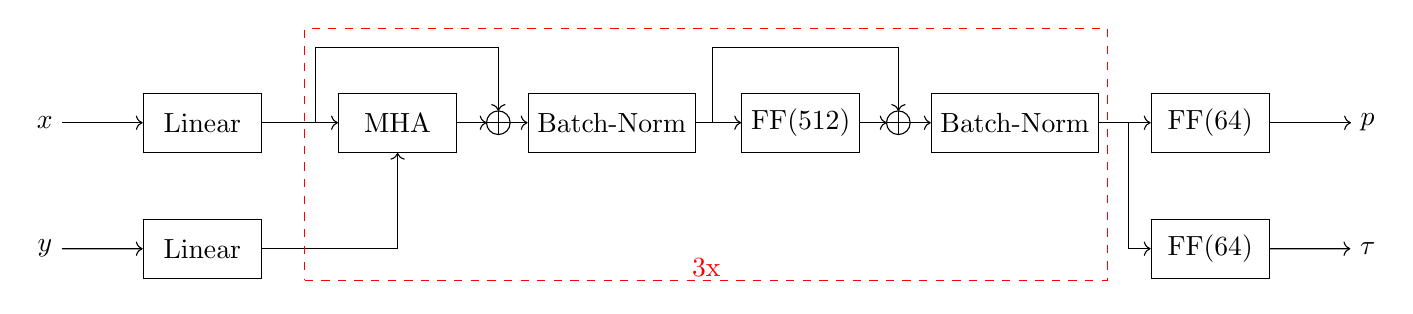
\begin{tikzpicture}[scale=0.8]
		\node at (0,0) (x) {$x$};
		\node[layer] at (2.5,0) (linx) {Linear};
		\node at (0,-2) (y) {$y$};
		\node[layer] at (2.5,-2) (liny) {Linear};
		\node[layer] at (5.6,0) (mha) {MHA};
		\node[plus] at (7.2,0) (skip-mha) {};
		\node[layer] at (9,0) (bn-mha) {Batch-Norm};
		\node[layer] at (12,0) (ff) {FF(512)};
		\node[plus] at (13.55,0) (skip-ff) {};
		\node[layer] at (15.4,0) (bn-ff) {Batch-Norm};
		\node[layer] at (18.5,0) (ffp) {FF(64)};
		\node at (21,0) (p) {$p$};
		\node[layer] at (18.5,-2) (fff) {FF(64)};
		\node at (21,-2) (f) {$\tau$};

		\draw[->] (x) -- (linx);
		\draw[->] (linx) -- (mha);
		\draw[->] (y) -- (liny);
		\draw[->] (liny) -| (mha);
		\draw[->] (mha) -- (skip-mha);
		\draw[->] (linx) -| ++(1.8,1.2) -| (skip-mha);
		\draw[->] (skip-mha) -- (bn-mha);
		\draw[->] (bn-mha) -- (ff);
		\draw[->] (ff) -- (skip-ff);
		\draw[->] (bn-mha) -| ++(1.6,1.2) -| (skip-ff);
		\draw[->] (skip-ff) -- (bn-ff);
		\draw[->] (bn-ff) -- (ffp);
		\draw[->] (ffp) -- (p);
		\draw[->] (bn-ff) ++(1.8,0) |- (fff);
		\draw[->] (fff) -- (f);

		\node[rectangle, draw=red, dashed, minimum width=10.2cm, minimum height=3.2cm] at (10.5,-0.5) {};
		\node[text=red] at (10.5, -2.3) {3x};
		\end{tikzpicture}
	}
	\captionof{figure}{Architecture of the GNN.}
	\end{centering}
	% cSpell:enable

	\important{MHA:} Multi-head attention, i.e., transformer-based convolution layer with 8 heads

	\bigskip
	$f_\Theta$ returns TTWP with maximal $p$ and rounded $\tau$
\end{frame}

\begin{frame}
	\frametitle{Training}
	Offline, in supervised fashion using representative problem instances

	\bigskip
	\structure{Collecting training samples:}

	\medskip
	\begin{enumerate}
	\itemsep2ex
	\item \important{Run Logic-based Benders Decomposition}
		\begin{itemize}
		\item enumerate \important{\emph{all} irreducible cuts} via MARCO, add them to the MP
		\item record all SPs and cuts
		\end{itemize}
	\item Determine a minimal subset of \important{\bf strong cuts},\\
		i.e., cuts actually required in MP to get feasible optimal solution
	\item For each subproblem: \important{Rollouts}
		\begin{itemize}
		\item Start with empty set $S$
		\item Successively add TTWPs leading to a strong cut randomly until $S$ $\widehat{=}$ irreducible cut
		\item \important{Each iteration:} add \important{training sample}
		\item \important{Labels:} based on strong cuts
		\end{itemize}
	\end{enumerate}

	\bigskip
	Loss function: binary cross-entropy
\end{frame}




\begin{frame}[fragile]
	\frametitle{Experiments Setup}
	\begin{itemize}
	\item \important{Instances} like in \emph{Horn, Raidl, and Rönnberg (2021)}, $n\in\{10,15,20,25\}$ tasks
	\item \verb|pytorch_geometric|, Gurobi 9.5, CP\,Optimizer 20.1
	\item AMD Ryzen 9 5900X
	\item For each $n$: 300\,000 to 600\,000 training samples from 2.000 to 200\,000 instances
	\item 40 to 300 training epochs
	\vspace{6mm}
	\item Comparison to \important{deletion filter} with different orders:
		\begin{itemize}
		\item Random
		\item Sorted: natural order from instance
		\item \citet{2013_coban-hooker_article}: sorted by decreasing slack
		\end{itemize}
	\end{itemize}
\end{frame}

\begin{frame}
	\frametitle{Results: Number of Solved SPs to Reach Optimality}
	\centering
	\cumuldistr{csv/avionics20_inst20}{no_subproblems_performed}{0.8\textwidth}{0.6\textheight}{\# of solved subproblems}{\# of solved\\instances}{\normalsize 20 Tasks}
	\ref{legend:cumuldistr-csv/avionics20_inst20-no_subproblems_performed}

	\bigskip
	Reduction: $\approx 70\%$
\end{frame}

\begin{frame}
	\frametitle{Results: Time to Reach Optimality}
	\centering
	\cumuldistr{csv/avionics20_inst20}{time_spent}{0.8\textwidth}{0.6\textheight}{Time {[s]}}{\# of solved\\instances}{}\hfill
	\ref{legend:cumuldistr-csv/avionics20_inst20-time_spent}

	\bigskip
	Reduction: $\approx 50\%$
\end{frame}

\begin{frame}
	\frametitle{Results: Number of MP Iterations}
	\centering
	\cumuldistr{csv/avionics20_inst20}{no_benders_iteration}{0.8\textwidth}{0.6\textheight}{Time {[s]}}{\# of LBBD iterations}{}\hfill
	\ref{legend:cumuldistr-csv/avionics20_inst20-no_benders_iteration}
\end{frame}

\begin{frame}{Results: Bounds over Time}
	\centering
	\includegraphics[width=10cm]{graphics/results-bounds.png}\hfill
	\ref{legend:cumuldistr-csv/avionics20_inst20-no_benders_iteration}
\end{frame}

\begin{frame}{Results: Out-of-Distribution Usage of GNNs}
	\centering
	25 Tasks\\
	\includegraphics[width=15cm]{graphics/results-extrapolation.png}
\end{frame}

\section{Conclusion}

\begin{frame}
	\frametitle{Conclusion and Future Work}
	\begin{itemize}
	\itemsep1.5ex
	\item \important{GNN} to \important{guide cut strengthening} in Logic-based Benders Decomposition
	\item Reduced \# subproblems to be solved by $\approx 70\%$
	\item Reduced runtime by $\approx 50\%$
	\item Promising future work
		\begin{itemize}
		\item Application to other/more complex problems
		\item Deeper analysis of importance of features, GNN structure
		\item Curriculum learning
		\item Reinforcement learning
		\end{itemize}
	\end{itemize}
\end{frame}




\begin{frame}[allowframebreaks]
	\frametitle{References}
	\footnotesize
	%\nocite{*} 
	% \bibliographystyle{abbrv}
	\bibliographystyle{apalike}
	\bibliography{lit.bib}
\end{frame}



\end{document}

